\documentclass[assignment = 1]{homework}

\usepackage{caption, subcaption, pdfpages, float}
\usepackage{graphics, wrapfig, pgf, graphicx}
\usepackage{enumitem}
\graphicspath{{../}}


% pacotes para importar código
\usepackage{caption, booktabs}
\usepackage[section, newfloat]{minted}
\definecolor{sepia}{RGB}{252,246,226}
\setminted{
    bgcolor = sepia,
    style   = pastie,
    frame   = leftline,
    autogobble,
    samepage,
    python3,
}
\setmintedinline{
    bgcolor={}
}

% ambientes de códigos de Python
\newmintedfile[pyinclude]{python}{}
\newmintinline[pyline]{python}{}
\newcommand{\pyref}[2]{\href{#1}{\texttt{#2}}}

\SetupFloatingEnvironment{listing}{name=Código}
\captionsetup[listing]{position=below,skip=-1pt}

\usepackage{csquotes}
\usepackage[style=verbose-ibid,autocite=footnote,notetype=foot+end,backend=biber]{biblatex}
\addbibresource{referencias.bib}
\usepackage[section]{placeins}

\usepackage[hidelinks]{hyperref}
\usepackage[noabbrev, nameinlink, brazilian]{cleveref}
\hypersetup{
    pdftitle  = {MC920 - Trabalho 1 - 187679},
    pdfauthor = {Tiago de Paula}
}

\newcommand{\textref}[2]{
    \hyperref[#2]{#1 \ref*{#2}}
}

\usepackage{import}
\usepackage{tikz}
\usetikzlibrary{matrix}
\usetikzlibrary{positioning}

\newenvironment{kmatrix}{
    \begin{tikzpicture}[node distance=0cm]
        \tikzset{square matrix/.style={
                matrix of nodes,
                column sep=-\pgflinewidth, row sep=-\pgflinewidth,
                nodes={draw,
                    minimum height=0.7cm,
                    anchor=center,
                    text width=0.7cm,
                    align=center,
                    inner sep=0pt
                },
            },
            square matrix/.default=0.7cm
        }
}{
    \end{tikzpicture}%
}

\newcommand*{\Scale}[2][4]{\scalebox{#1}{\ensuremath{#2}}}%


\begin{document}

    \pagestyle{main}

    \section{Introdução}

Este trabalho teve como objetivo a implementação e a análise de alguns filtros de imagem no domínio espacial. A filtragem é feita pela convolução da imagem com uma máscara utilizando bibliotecas de processamento de imagens.

A \cref{fig:base} apresenta as imagens base deste trabalho, usadas para análise e discussão dos filtros. Todas elas são monocromáticas. Os filtros utilizados serão apresentados ao longo do relatório, à medida que forem necessários pelo texto.

\begin{figure}[H]
    \centering
    \begin{subfigure}{0.33\textwidth}
    \centering
    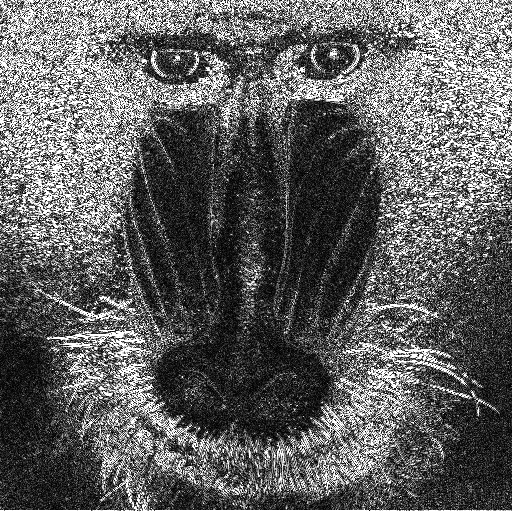
\includegraphics[width=4.4cm]{imagens/baboon.png}
    \caption{\texttt{imagens/baboon.png}}
\end{subfigure}%
\begin{subfigure}{0.33\textwidth}
    \centering
    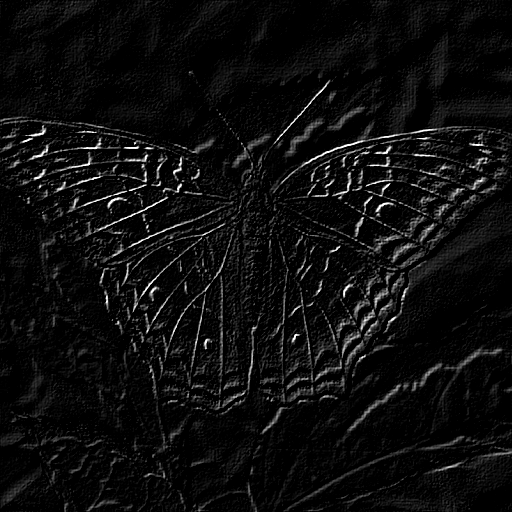
\includegraphics[width=4.4cm]{imagens/butterfly.png}
    \caption{\texttt{imagens/butterfly.png}}
\end{subfigure}\\[8pt]
\begin{subfigure}{0.33\textwidth}
    \centering
    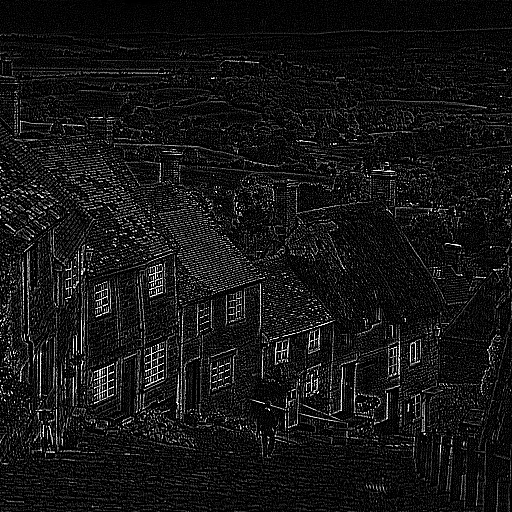
\includegraphics[width=4.4cm]{imagens/city.png}
    \caption{\texttt{imagens/city.png}}
\end{subfigure}%
\begin{subfigure}{0.33\textwidth}
    \centering
    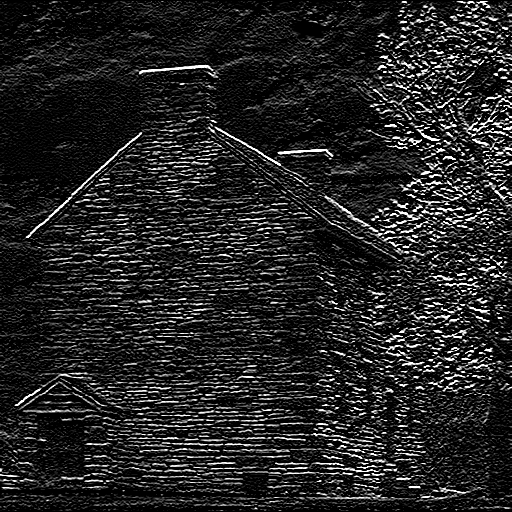
\includegraphics[width=4.4cm]{imagens/house.png}
    \caption{\texttt{imagens/house.png}}
\end{subfigure}%
\begin{subfigure}{0.33\textwidth}
    \centering
    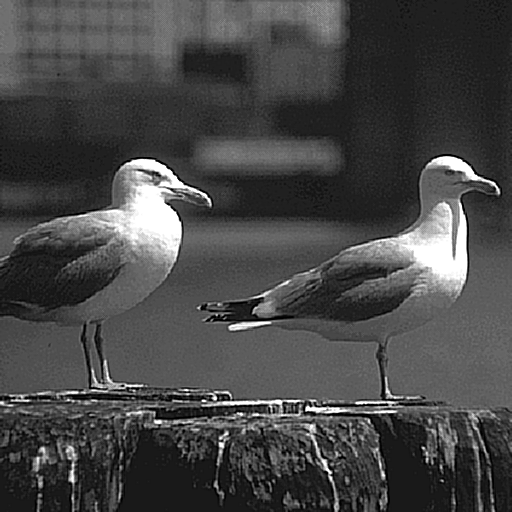
\includegraphics[width=4.4cm]{imagens/seagull.png}
    \caption{\texttt{imagens/seagull.png}}
\end{subfigure}

    \caption{Imagens base da comparação dos filtros.}
    \label{fig:base}
\end{figure}


    \section{O Programa}

Além das bibliotecas padrão de Python, foram utilizados os pacotes SciPy \autocite{ref:scipy} e OpenCV \autocite{ref:opencv}.

\subsection{Código Fonte}

    O programa foi desenvolvido em Python 3.8, mas deveria funcionar com as versões 3.6 e 3.7 também. Além disso, o código fonte foi separado nos seguintes arquivos:

    \begin{description}
        \item[main.py] É o corpo do programa, resposável por processar os comandos e opções da linha de comando.

        \item[lib.py] Funções de tranformação da imagem, como ajuste de brilho e acesso do plano de bits.

        \item[filtro.py] Definição das máscaras de convoluções (\textit{kernels}).

        \item[inout.py] Funções que tratam da entrada e saída do programa, como leitura e escrita de arquivos de imagem e também da apresentação da imagem em uma janela gráfica.

        \item[tipos.py] Definição dos tipos para checagem estática com \texttt{mypy} \autocite{ref:mypy}.
    \end{description}

    Todas as figuras base utilizadas neste relatório podem ser encontradas na pasta \texttt{imagens} do código fonte, como descrito nos rótulos da \cref{fig:base}. Além disso, foi disponibilizado também um \textit{script} em \texttt{bash}, \texttt{run.sh}, que realiza todos os processamentos requeridos em cada uma das imagens na pasta.

\subsection{Execução}

    A execução deve ser feita através do interpretador de Python 3.6+. A única entrada obrigatória é o caminho para a imagem PNG que será processada. As entradas seguintes devem ser os \textit{kernels} de convolução, no formato \texttt{h1} até \texttt{h11}. Ao final da execução, a imagem resultante será exibida na tela. Por exemplo, o comando abaixo apresenta a \cref{fig:execucao} em uma nova janela gráfica.

    \begin{minted}{text}
        $ python3 main.py imagens/baboon.png h1 h2
    \end{minted}

    \begin{figure}[H]
        \centering
        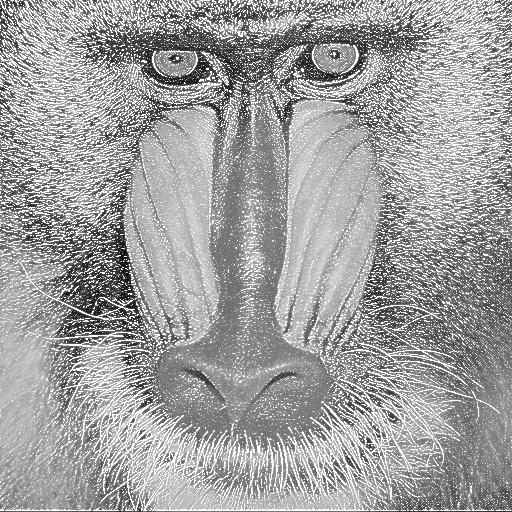
\includegraphics[width=6cm]{resultados/execucao.png}

        \caption{Aplicação de alguns processamentos na \texttt{baboon.png}.}
        \label{fig:execucao}
    \end{figure}

    Além das entradas posicionais, existem algums argumentos opicionais, que podem ser vistos com \mintinline{bash}{$ python3 main.py --help}. A mais importante das opções é \mintinline{text}{--output}, ou \mintinline{text}{-o}, que salva o resultado em um arquivo PNG em vez de exibir na tela. Se é desejável tanto a exibição da imagem quanto o salvamento no arquivo, o argumento \mintinline{text}{--force-show} ou \mintinline{text}{-f} pode ser usado. As outras opções são referentes ao processamento das imagens e serão descritas na seção seguinte.


    \section{Implementação} \label{sec:impl}

\subsection{Teoria: Correlação e Convolução}

    A correlação é uma operação em que os pesos são aplicados na ordem em que aparecem visualmente. Assim, considerando o produto Hadamard ($\bar{\cdot}$),  a correlação ($\circ$) de uma região $R$ da imagem por uma máscara $M$ (de dimensões $N \times N$) será \autocite{ref:corrconv}:

\begin{equation*}
    R \circ M = \sum_{i = 1}^N \sum_{j = 1}^N R_{i,j} M_{i,j} = \sum_{i = 1}^N \sum_{j = 1}^N \left(R \,\bar{\cdot}\, M\right)_{i,j}
\end{equation*}

Portanto, a implementação dessa etapa em NumPy poderia ser:

\begin{minted}{python}
    def correlacao_regiao(R: np.ndarray, M: np.ndarray) -> float:
        return np.sum(R * M)
\end{minted}

Podemos ver isso mais visualmente com o seguinte exemplo de um filtro $3 \times 3$ em uma região genérica.

\begin{equation*}
    \begin{bmatrix}
        a & b & c \\
        d & e & f \\
        g & h & k
    \end{bmatrix} \circ \begin{bmatrix}
        0 & 1 & 0 \\
        2 & 3 & 1 \\
        0 & 0 & 0
    \end{bmatrix}
    = b + 2d + 3e + f
\end{equation*}

Apesar disso, a problema pedia a implementação de uma convolução. Nesse processamento a ordem dos elementos de um dos sinais era percorrido de forma contrária, de modo que os sinais fossem combinados na mesma ordem em que aparecem visualmente. Podemos ver isso na \cref{fig:convolucao-sinal}, onde a reflexão do eixo em $g(-\tau)$ faz com que os primeiros pontos de $g(t)$ sejam combinados antes, isto é, $g(t=1)$ aparece antes de $g(t=4)$ na varredura apresentada nos três últimos gráficos.

Com a mesma região $R$ e máscara $M$ acima, a convolução discreta resulta em \autocite{ref:corrconv}:

\begin{equation*}
    R \ast M = \sum_{i = 1}^N \sum_{j = 1}^N R_{i,j} M_{N-i,N-j} \ne R \circ M
\end{equation*}

Observando o exemplo matricial anterior, teremos o seguinte comportamento.

\begin{equation} \label{eq:corrconv}
    \begin{bmatrix}
        a & b & c \\
        d & e & f \\
        g & h & k
    \end{bmatrix} \ast \begin{bmatrix}
        0 & 1 & 0 \\
        2 & 3 & 1 \\
        0 & 0 & 0
    \end{bmatrix}
    = d + 3e + 2f + h =
    \begin{bmatrix}
        a & b & c \\
        d & e & f \\
        g & h & k
    \end{bmatrix} \circ \begin{bmatrix}
        0 & 0 & 0 \\
        1 & 3 & 2 \\
        0 & 1 & 0
    \end{bmatrix}
\end{equation}

A convolução é comumente usada devido a familiaridade das vastas propriedades dessa operação. Por outro lado, a correlação também aparece em vários processamentos de imagem devido à sua aproximação com a visualização de matrizes.

\begin{figure}[H]
    \centering
    \def\svgwidth{12cm}
    \input{figuras/convolucao-sinal.pdf_tex}

    \caption{Exemplo visual da convolução em sinais unidimensionais contínuos.}
    \label{fig:convolucao-sinal}
\end{figure}


\subsection{Código da Convolução}

    A convolução foi implementada em dois \textit{beckends} distintos, com as funções \pyline{convolve} do SciPy \autocite{ref:ndimage} e \pyline{filter2D} do OpenCV \autocite{ref:cvfilter}. A função dos SciPy realiza uma convolução, como definida matematicamente e foi implementada como no \textref{código}{code:scipy}, ignorando o tratamento das bordas.

\begin{listing}[H]
    \begin{minted}{python}
        import numpy as np
        from scipy import ndimage

        def scipy_convolve(input: Image, kernel: Kernel, borda: ...) -> np.ndarray:
            # mudança para float
            input = input.astype(np.float64)
            # convolução
            output = ndimage.convolve(input, kernel, ...)
            return output
    \end{minted}

    \caption{Convolução com o SciPy, sem o tratamento de bordas.}
    \label{code:scipy}
\end{listing}

A biblioteca OpenCV não tem uma operação de convolução, considerando a definição formal. Assim, a função \pyline{cv2.filter2D} faz realmente uma correlação.

Como podemos ver na \cref{eq:corrconv}, as duas operações são similares, bastando reverter a posição dos elementos de uma das matriz. A máscara normalmente é bem menor em relação à imagem, então ela que foi invertida. No caso do OpenCV, esse tipo de inversão das posições, de $(i, j)$ para $(N-i, N-j)$, pode ser feito pelo \pyline{cv2.flip} \autocite{ref:cvflip}, com o argumento \pyline{flipCode} negativo. A implementação da convolução, nesse caso, ficou como no \textref{código}{code:opencv}.

\begin{listing}[H]
    \begin{minted}{python}
        import numpy as np
        import cv2

        def opencv_convolve(input: Image, kernel: Kernel, borda: ...) -> np.ndarray:
            # flip do kernel para a correlação equivalente
            kernel = cv2.flip(kernel, flipCode=-1)
            # convolução
            output = cv2.filter2D(input, cv2.CV_64F, kernel, ...)
            return output
    \end{minted}

    \caption{Convolução com o OpenCV, sem o tratamento de bordas.}
    \label{code:opencv}
\end{listing}

Para selecionar entre os \textit{backends}, existem dois argumentos opcionais. O \mintinline{bash}{--scipy} garante a execução com a biblioteca SciPy, por mais que já seja o padrão. Podemos então conseguir a mesma imagem da \cref{fig:execucao} com o comando:

\begin{minted}{bash}
    $ python3 main.py imagens/baboon.png h1 h2 --scipy
\end{minted}

Do mesmo modo, o OpenCV pode ser escolhido com o argumento \mintinline{bash}{--opencv}.

\begin{minted}{bash}
    $ python3 main.py imagens/baboon.png h1 h2 --opencv
\end{minted}


\subsection{Tratamento de Bordas}

    \begin{figure}[H]
        \centering
        \begin{figure}[H]
    \centering
    \begin{subfigure}{0.48\textwidth}
        \centering
        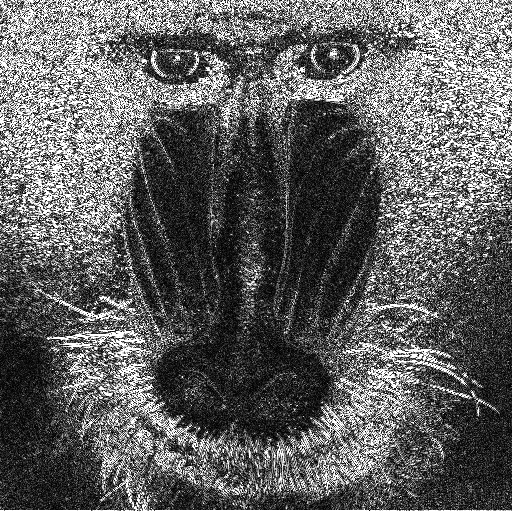
\includegraphics[width=0.9\textwidth]{imagens/baboon.png}
        \caption{Original: \texttt{baboon.png}.}
    \end{subfigure}\\[8pt]
    \begin{subfigure}{0.48\textwidth}
        \centering
        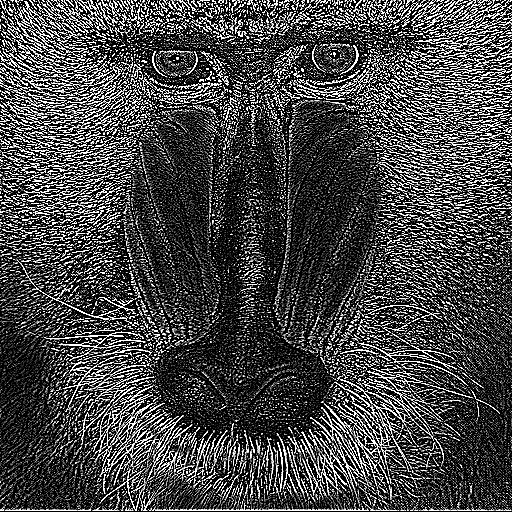
\includegraphics[width=0.9\textwidth]{resultados/baboon_h1.png}
        \caption{Convolução com $h_1$ (\ref{fig:h1}).}
        \label{fig:borda:viz4}
    \end{subfigure}%
    \begin{subfigure}{0.48\textwidth}
        \centering
        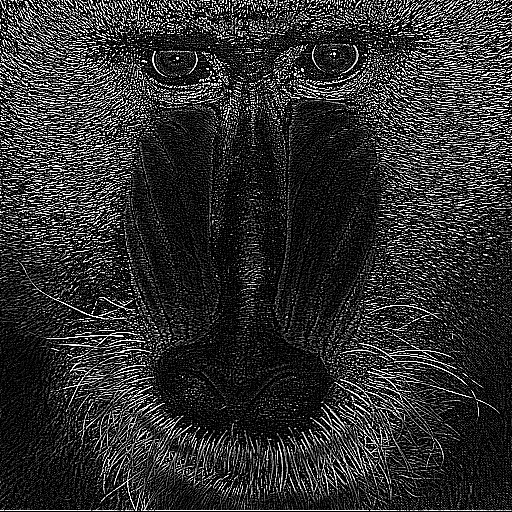
\includegraphics[width=0.9\textwidth]{resultados/baboon_h5.png}
        \caption{Convolução com $h_5$ (\ref{fig:h5}).}
        \label{fig:borda:viz8}
    \end{subfigure}

    \caption{Aplicação do laplaciano discreto.}
\end{figure}

Os filtros de detecção ou realce de bordas mais comuns são os chamados não-direcionais. Normalmente, eles são desenvolvidos a partir do operador laplaciano discreto \autocite{ref:laplacian}. Uma característica importante dos filtros de detecção de bordas é que seus elementos somam zero.

O operador laplaciano serve como uma medida de quanto uma função espacial no ponto $p$ é diferente da média dos pontos em um raio $[p - \delta r, p + \delta r]$. No caso discreto bidimensional, como imagens, existem duas principais medidas de distância, considerando as vizinhaças 4 e 8. Elas resultam em dois tipos de laplacianos diferentes, como pode ser visto na \cref{fig:borda:kernel}.

Nesse trabalho temos o \textit{kernel} $h_1$ (\ref{fig:h1}), com vizinhaça 4 de raio 2, e o $h_5$, com vizinhaça 8 de raio 1. Os resultados podem ser vistos nas figuras \ref{fig:borda:viz4} e \ref{fig:borda:viz8}, respectivamente. Podemos ver que as bordas nas regiões de baixa frequência são bem detectadas, como no centro da imagem, mas regiões de alta frequência resultam em muita informação e podem acabar atrapalhando a análise das bordas. Uma forma de contornar esse problema é aplicando um filtro passa-baixas, como o \textit{blur} gaussiano, discutido na \cref{sec:blur}.

\begin{figure}[H]
    \centering
    \begin{subfigure}{0.4\textwidth}
        \centering
        \begin{kmatrix}
    \matrix[square matrix]{
        0 & 0 & -1 & 0 & 0 \\
        0 & -1 & -2 & -1 & 0 \\
        -1 & -2 & 16 & -2 & -1 \\
        0 & -1 & -2 & -1 & 0 \\
        0 & 0 & -1 & 0 & 0 \\
    };
\end{kmatrix}
        \caption{~$h_1$}
        \label{fig:h1}
    \end{subfigure}%
    \begin{subfigure}{0.4\textwidth}
        \centering
        \begin{kmatrix}
    \matrix[square matrix]{
        -1 & -1 & -1 \\
        -1 & 8 & -1 \\
        -1 & -1 & -1 \\
    };
\end{kmatrix}
        \caption{~$h_5$}
        \label{fig:h5}
    \end{subfigure}

    \caption{Filtros laplacianos discretos}
    \label{fig:borda:kernel}
\end{figure}

A execução pode ser feita com:

\begin{minted}{bash}
    $ python3 main.py imagens/baboon.png h1
    # ou
    $ python3 main.py imagens/baboon.png h5
\end{minted}


        \caption{Argumentos válidos para \mintinline{bash}{--borda} ou \mintinline{bash}{-b}.}
        \label{fig:borda}
    \end{figure}

    Para que a convolução possa ser feita nas bordas da imagem, existem vários modos de tratamento. Na ferramenta foram implementadas três formas de dentre as várias possíveis: a extensão do último pixel (\ref{fig:borda:extensao}), a reflexão dos pixels de borda (\ref{fig:borda:reflexao}) e a mesma reflexão, mas sem repetir o pixel mais externo (\ref{fig:borda:reflexao-pulada}).

    A \textit{flag} \mintinline{bash}{--borda}, ou \mintinline{bash}{-b}, serve para controlar o tratamento de borda. As opções devem ser passadas como aparecem na \cref{fig:borda}. Por padrão, o tratamento é feito como na \cref{fig:borda:reflexao-pulada}, como se fosse a opção \mintinline{bash}{-b reflexao_pula_ultimo}. Ambos \textit{backends}, SciPy e OpenCV, funcionam com os três tipos de bordas.

    Apesar de interessante, e em alguns casos importante, o três tratamentos de bordas não alteram muito no resultado da convolução. A razão disso é que os \textit{kernels} desse trabalho são relativamente pequenos.

\subsection{Discretização}

    Toda o processo de convolução é feito com operações de ponto flutuante, buscando evitar \textit{overflow} e problemas de arredondamento. Então, para que a matriz volte a representar uma imagem, é preciso discretizar os valores, para os níveis 0 a 255.

    A forma mais comum é arrendondando os valores para os inteiros mais próximos no intervalo $[0, 255]$. Dessa forma, os valores negativos se tornam 0 e valores maiores que 255 vão para 255. No código, esse método foi implementado na função \pyline{lib.trunca}. Essa é a opção padrão do programa.

    Uma forma alternativa também foi implementada, baseada no mapeamento linear do menor valor da imagem para 0 e do maior para 255. Na ferramenta em Python, esse método de discretização está implementado na função \pyline{lib.transforma_limites} e pode ser selecionada com a opção \mintinline{bash}{-t} na linha de comando. Essa opção não foi muito utilizada neste relatório.

\subsection{Combinação das Imagens}

    Vários filtros podem ser passados como argumento, como no exemplo da \cref{sec:execucao}. Os filtros são aplicados, um por vez, na mesma imagem de entrada, discretizados e só então combinados em uma imagem final. A combinação é feita pela raiz da soma quadrática, em ponto flutuante, e discretizada novamente.

    Para padronizar a implementação, a etapa de combinação é feita mesmo com apenas uma imagem. Por causa disso, a discretização é feita antes e depois da combinação, mantendo o resultado esperado da convolução. No entanto, isso pode ser alterado com a opção \mintinline{bash}{-n}, fazendo com que a discretização seja aplicada apenas no final.

    Para um filtro apenas, isso faz com que a convolução seja tratada pelo valor absoluto, fazendo as imagens ficarem com regiões mais claras, onde anteriormente seria preto. Esse modo não foi utilizado neste relatório.


    \section{Resultados}

\subsection{Blur} \label{sec:blur}

    Os filtros mais simples de identificar foram os de \textit{blur}, que fazem um tipo de média ponderada da vizinhaça do pixel.

\begin{figure}[H]
    \centering
    \begin{subfigure}{0.4\textwidth}
        \centering
        \begin{kmatrix}
    \matrix(img)[square matrix]{
        1 & 4 & 6 & 4 & 1 \\
        4 & 6 & 24 & 6 & 4 \\
        6 & 24 & 36 & 24 & 6 \\
        4 & 6 & 24 & 6 & 4 \\
        1 & 4 & 6 & 4 & 1 \\
    };

    \node[left=of img] {$\displaystyle\Scale[1.7]{\frac{1}{256}}$};
\end{kmatrix}
        \caption{~$h_2$}
        \label{fig:h2}
    \end{subfigure}%
    \begin{subfigure}{0.4\textwidth}
        \centering
        \begin{kmatrix}
    \matrix(img)[square matrix]{
        1 & 1 & 1 \\
        1 & 1 & 1 \\
        1 & 1 & 1 \\
    };

    \node[left=of img] {$\displaystyle\Scale[1.7]{\frac{1}{9}}$};
\end{kmatrix}
        \caption{~$h_6$}
        \label{fig:h6}
    \end{subfigure}

    \caption{Máscaras de \textit{blur}.}
    \label{fig:blur:kernel}
\end{figure}

O primeiro deles é o filtro gaussiano $5 \times 5$ \autocite{ref:gaussian}, que pode ser visto na \cref{fig:h2}. Essa matriz é ponderada de acordo com as distâncias 4 do pixel central, reduzindo o peso para pixels mais distantes. No espaço das frequências, esse filtro funciona como um passa-baixas, reduzindo a influência de frequências muito altas, o que pode servir para melhorar o resultado de outros filtros, como o laplaciano, ou para evitar problemas de \textit{aliasing} \autocite{ref:gaussian-lowpass}. Na \cref{fig:blur:gauss}, podemos ver o resultado de aplicar esse filtro na imagem \texttt{house.png} (\ref{fig:blur:orig}).

\begin{figure}[H]
    \centering
    \begin{subfigure}{0.48\textwidth}
        \centering
        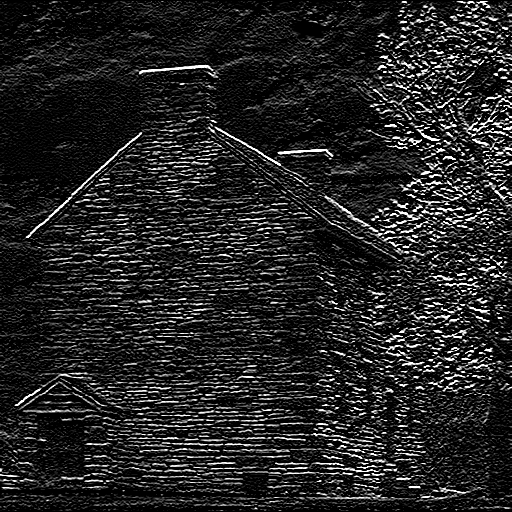
\includegraphics[width=0.9\textwidth]{imagens/house.png}
        \caption{Original: \texttt{house.png}.}
        \label{fig:blur:orig}
    \end{subfigure}\\[8pt]
    \begin{subfigure}{0.48\textwidth}
        \centering
        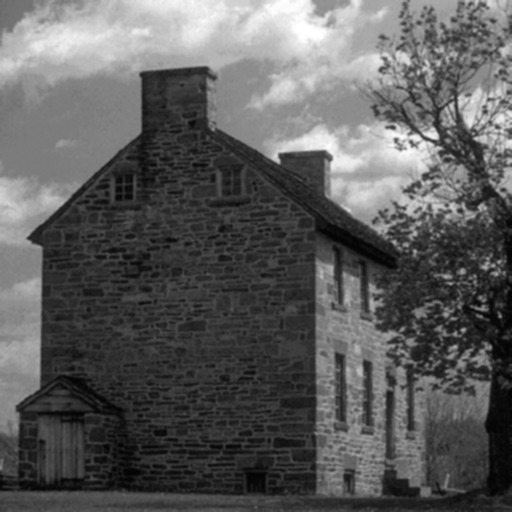
\includegraphics[width=0.9\textwidth]{resultados/house_h2.png}
        \caption{Convolução com $h_2$ (\ref{fig:h2}).}
        \label{fig:blur:gauss}
    \end{subfigure}%
    \begin{subfigure}{0.48\textwidth}
        \centering
        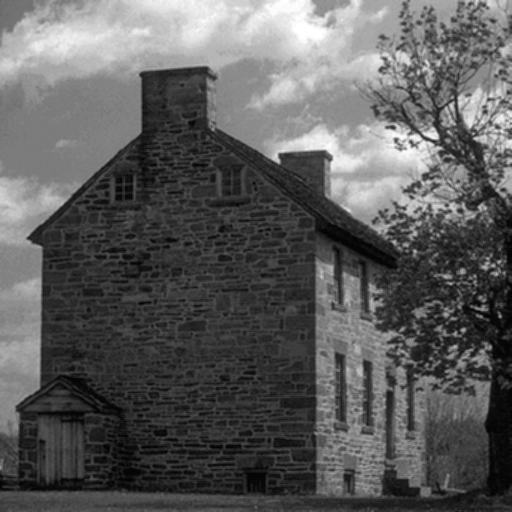
\includegraphics[width=0.9\textwidth]{resultados/house_h6.png}
        \caption{Convolução com $h_6$ (\ref{fig:h6}).}
        \label{fig:blur:box}
    \end{subfigure}

    \caption{Aplicação do \textit{blur}.}
    \label{fig:blur}
\end{figure}

O segundo filtro é chamada de \textit{box blur}, que faz uma média simples da vizinhaça 8 do pixel. Isso pode ser visto no \textit{kernel} do filtro (\cref{fig:h6}). Apesar de ser diferente do gaussiano, o resultado ficou bem parecido, como pode ser visto na \cref{fig:blur}. O motivo disso é que os pesos mais externos do filtro gaussiano $5 \times 5$ são bem baixos, fazendo com a região $3 \times 3$ seja mais presente, sendo essa a mesma região do filtro \textit{box}.

No programa, esses filtros podem ser aplicados com: \enlargethispage{20pt}

\begin{minted}{bash}
    $ python3 main.py imagens/house.png h2 # ou h6
\end{minted}


\subsection{Motion Blur} \label{sec:motion}

    % http://users.ece.northwestern.edu/~sda690/MfB/Motion_CVPR08.pdf
% https://www.geeksforgeeks.org/opencv-motion-blur-in-python/
% https://www.wikiwand.com/en/Motion_blur
% http://tech.abdulfatir.com/2014/05/kernel-image-processing.html

Além dos filtros de \textit{blur} apresentados na \hyperref[sec:blur]{seção anterior}, temos também um filtro de \textit{blur} direcionado, muitas vezes usado para alcançar um efeito de \textit{motion blur}. Para o \textit{kernel} da \cref{fig:h9}, o \textit{blur} está direcionado a 45\textdegree, como se a câmera estivesse se movendo da esquerda-superior para a direita-inferior.

\begin{figure}[H]
    \centering
    \begin{kmatrix}
    \matrix(img)[square matrix]{
        1 & 0 & 0 & 0 & 0 & 0 & 0 & 0 & 0 \\
        0 & 1 & 0 & 0 & 0 & 0 & 0 & 0 & 0 \\
        0 & 0 & 1 & 0 & 0 & 0 & 0 & 0 & 0 \\
        0 & 0 & 0 & 1 & 0 & 0 & 0 & 0 & 0 \\
        0 & 0 & 0 & 0 & 1 & 0 & 0 & 0 & 0 \\
        0 & 0 & 0 & 0 & 0 & 1 & 0 & 0 & 0 \\
        0 & 0 & 0 & 0 & 0 & 0 & 1 & 0 & 0 \\
        0 & 0 & 0 & 0 & 0 & 0 & 0 & 1 & 0 \\
        0 & 0 & 0 & 0 & 0 & 0 & 0 & 0 & 1 \\
    };

    \node[left=of img] {$\displaystyle\Scale[1.7]{\frac{1}{9}}$};
\end{kmatrix}

    \caption{Máscara de \textit{motion blur}: $h_9$.}
    \label{fig:h9}
\end{figure}

\begin{figure}[H]
    \centering
    \begin{subfigure}{0.48\textwidth}
        \centering
        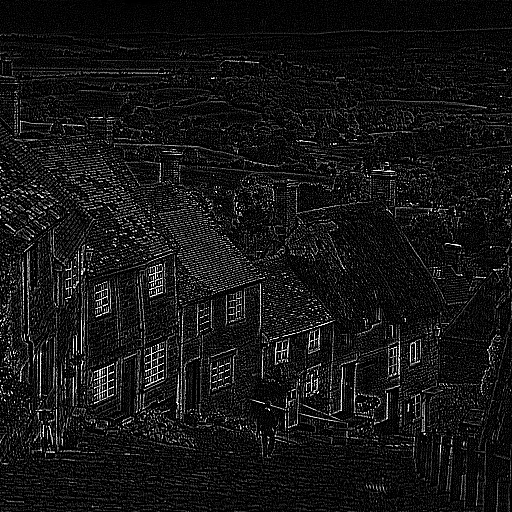
\includegraphics[width=0.9\textwidth]{imagens/city.png}
        \caption{Original: \texttt{city.png}.}
    \end{subfigure}%
    \begin{subfigure}{0.48\textwidth}
        \centering
        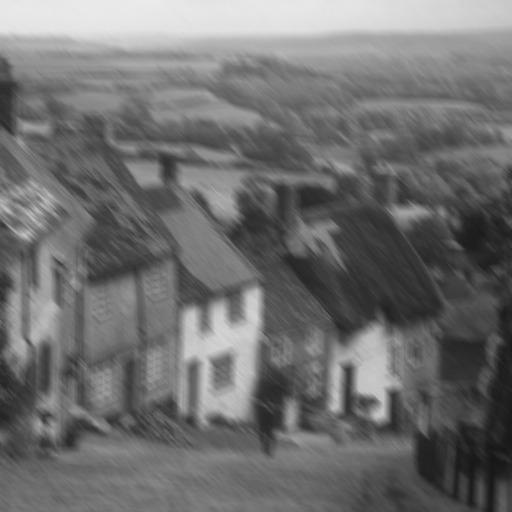
\includegraphics[width=0.9\textwidth]{resultados/city_h9.png}
        \caption{Convolução com $h_9$ (\ref{fig:h9}).}
        \label{fig:motion:conv}
    \end{subfigure}

    \caption{Aplicação de \textit{motion blur}.}
    \label{fig:motion}
\end{figure}

Para a execução pelo programa, o comando deve ser no formato abaixo, resultando em algo como a \cref{fig:motion:conv}.

\begin{minted}{bash}
    $ python3 main.py imagens/city.png h9
\end{minted}



\subsection{Detecção de Borda} \label{sec:borda}

    \begin{figure}[H]
    \centering
    \begin{subfigure}{0.48\textwidth}
        \centering
        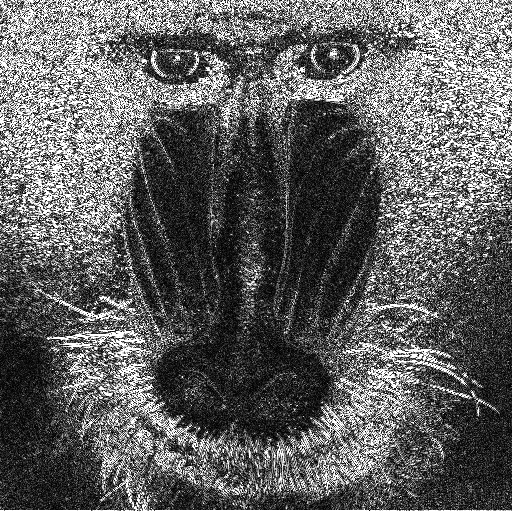
\includegraphics[width=0.9\textwidth]{imagens/baboon.png}
        \caption{Original: \texttt{baboon.png}.}
    \end{subfigure}\\[8pt]
    \begin{subfigure}{0.48\textwidth}
        \centering
        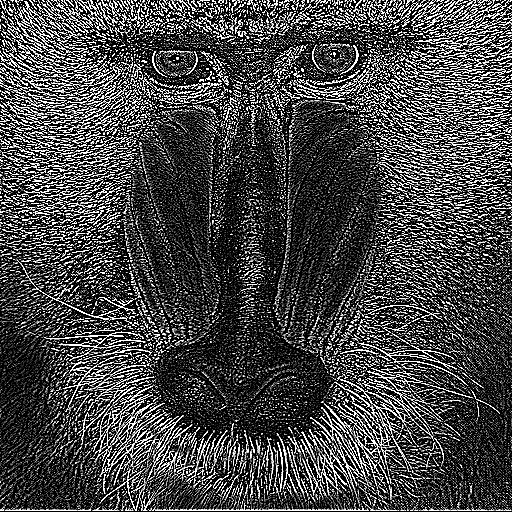
\includegraphics[width=0.9\textwidth]{resultados/baboon_h1.png}
        \caption{Convolução com $h_1$ (\ref{fig:h1}).}
        \label{fig:borda:viz4}
    \end{subfigure}%
    \begin{subfigure}{0.48\textwidth}
        \centering
        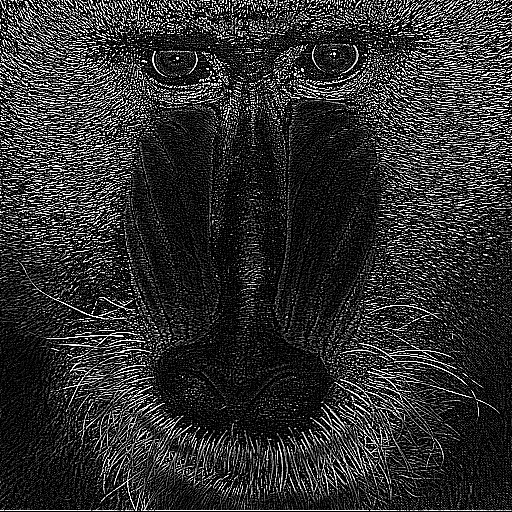
\includegraphics[width=0.9\textwidth]{resultados/baboon_h5.png}
        \caption{Convolução com $h_5$ (\ref{fig:h5}).}
        \label{fig:borda:viz8}
    \end{subfigure}

    \caption{Aplicação do laplaciano discreto.}
\end{figure}

Os filtros de detecção ou realce de bordas mais comuns são os chamados não-direcionais. Normalmente, eles são desenvolvidos a partir do operador laplaciano discreto \autocite{ref:laplacian}. Uma característica importante dos filtros de detecção de bordas é que seus elementos somam zero.

O operador laplaciano serve como uma medida de quanto uma função espacial no ponto $p$ é diferente da média dos pontos em um raio $[p - \delta r, p + \delta r]$. No caso discreto bidimensional, como imagens, existem duas principais medidas de distância, considerando as vizinhaças 4 e 8. Elas resultam em dois tipos de laplacianos diferentes, como pode ser visto na \cref{fig:borda:kernel}.

Nesse trabalho temos o \textit{kernel} $h_1$ (\ref{fig:h1}), com vizinhaça 4 de raio 2, e o $h_5$, com vizinhaça 8 de raio 1. Os resultados podem ser vistos nas figuras \ref{fig:borda:viz4} e \ref{fig:borda:viz8}, respectivamente. Podemos ver que as bordas nas regiões de baixa frequência são bem detectadas, como no centro da imagem, mas regiões de alta frequência resultam em muita informação e podem acabar atrapalhando a análise das bordas. Uma forma de contornar esse problema é aplicando um filtro passa-baixas, como o \textit{blur} gaussiano, discutido na \cref{sec:blur}.

\begin{figure}[H]
    \centering
    \begin{subfigure}{0.4\textwidth}
        \centering
        \begin{kmatrix}
    \matrix[square matrix]{
        0 & 0 & -1 & 0 & 0 \\
        0 & -1 & -2 & -1 & 0 \\
        -1 & -2 & 16 & -2 & -1 \\
        0 & -1 & -2 & -1 & 0 \\
        0 & 0 & -1 & 0 & 0 \\
    };
\end{kmatrix}
        \caption{~$h_1$}
        \label{fig:h1}
    \end{subfigure}%
    \begin{subfigure}{0.4\textwidth}
        \centering
        \begin{kmatrix}
    \matrix[square matrix]{
        -1 & -1 & -1 \\
        -1 & 8 & -1 \\
        -1 & -1 & -1 \\
    };
\end{kmatrix}
        \caption{~$h_5$}
        \label{fig:h5}
    \end{subfigure}

    \caption{Filtros laplacianos discretos}
    \label{fig:borda:kernel}
\end{figure}

A execução pode ser feita com:

\begin{minted}{bash}
    $ python3 main.py imagens/baboon.png h1
    # ou
    $ python3 main.py imagens/baboon.png h5
\end{minted}


\subsection{Operador de Sobel} \label{sec:sobel}

    Além dos detectores de borda não-direcionais, existem detectores que se importam com qual direção está sendo feita a análise. Muitos desses operadores são baseados na noção de gradiente, que representa matematicamente exatamente essa ideia.

Dentre eles, existe o operador de Sobel \autocite{ref:sobel}, que faz o gradiente nas direções $x$ e $y$ do plano cartesiano. Em específico, considerando a operação de convolução, o filtro $h_3$ (\ref{fig:h3}) aponta na direção $-x$ (para a esquerda) e o $h_4$ (\ref{fig:h4}), na $-y$ (para cima).

\begin{figure}[H]
    \centering
    \begin{subfigure}{0.4\textwidth}
        \centering
        \begin{kmatrix}
    \matrix[square matrix]{
        -1 & 0 & 1 \\
        -2 & 0 & 2 \\
        -1 & 0 & 1 \\
    };
\end{kmatrix}
        \caption{~$h_3$}
        \label{fig:h3}
    \end{subfigure}%
    \begin{subfigure}{0.4\textwidth}
        \centering
        \begin{kmatrix}
    \matrix[square matrix]{
        -1 & -2 & -1 \\
        0 & 0 & 0 \\
        1 & 2 & 1 \\
    };
\end{kmatrix}
        \caption{~$h_4$}
        \label{fig:h4}
    \end{subfigure}

    \caption{Máscaras de Sobel.}
    \label{fig:sobel:kernel}
\end{figure}

Observando os resultados na \cref{fig:sobel}, podemos ver que quase não existe separação do corpo da borboleta com as asas na \cref{fig:sobel:y}, isso porque ela quase não apresenta variações verticais nessa região. Nessa mesma figura, no entanto, podemos ver claramente a separação do topo da asa, que não acontece na \cref{fig:sobel:x}, já que é uma região com pouca variaçao horizontal.

Além disso, podemos ver a presença do direcinamento $-x$ em vez do $+x$ na \ref{fig:sobel:x}. Em especial, na parte inferior da asa esquerda, logo abaixo do abdômen do inseto, é bem visível a borda do componente, o que não acontece na mesma região da asa direita. No tórax da borboleta também fica visível uma separação bilateral, que não é aparente na imagem original (\ref{fig:sobel:orig}).

Muitas vezes, os operadores de Sobel são combinados para extrair informações importantes do gradiente. O mais comum, é o módulo da gradiente, que no caso é encontrado por $\sqrt{\left(h_3\right)^2 + \left(h_4\right)^2}$. Ele serve como um bom detector de borda, medindo o quão forte é a variação em cada região da imagem. O resultado pode ser visto na \cref{fig:sobel:abs}.

\begin{figure}[H]
    \centering
    \begin{subfigure}{0.48\textwidth}
        \centering
        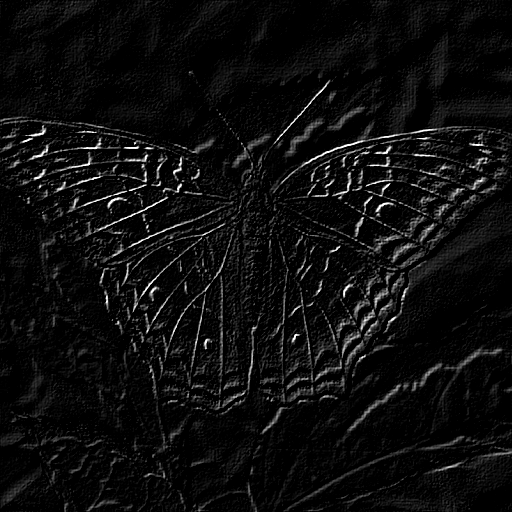
\includegraphics[width=0.9\textwidth]{imagens/butterfly.png}
        \caption{Original: \texttt{butterfly.png}.}
        \label{fig:sobel:orig}
    \end{subfigure}%
    \begin{subfigure}{0.48\textwidth}
        \centering
        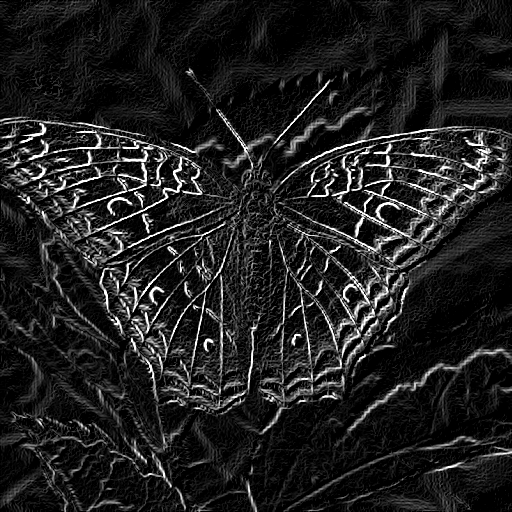
\includegraphics[width=0.9\textwidth]{resultados/butterfly_h3h4.png}
        \caption{Convolução com $h_3$ e $h_4$.}
        \label{fig:sobel:abs}
    \end{subfigure}\\[8pt]
    \begin{subfigure}{0.48\textwidth}
        \centering
        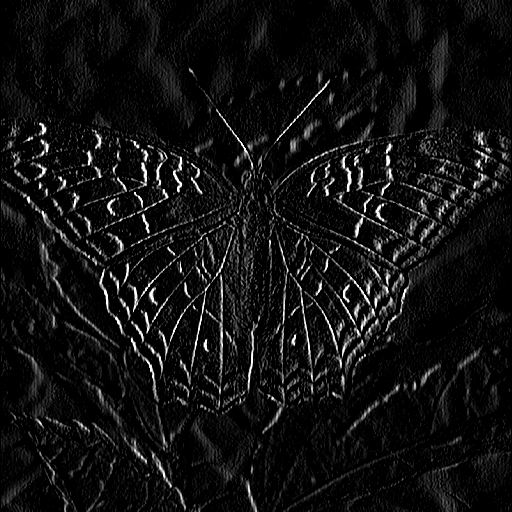
\includegraphics[width=0.9\textwidth]{resultados/butterfly_h3.png}
        \caption{Convolução com $h_3$.}
        \label{fig:sobel:x}
    \end{subfigure}%
    \begin{subfigure}{0.48\textwidth}
        \centering
        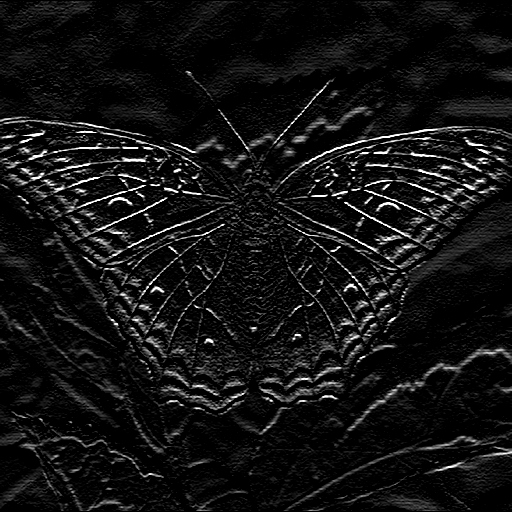
\includegraphics[width=0.9\textwidth]{resultados/butterfly_h4.png}
        \caption{Convolução com $h_4$.}
        \label{fig:sobel:y}
    \end{subfigure}

    \caption{Aplicação dos operadores de Sobel.}
    \label{fig:sobel}
\end{figure}

A aplicação do operador de Sobel, na forma mais completa, pode ser feita no programa por:

\begin{minted}{bash}
    $ python3 main.py imagens/butterfly.png h3 h4
\end{minted}


\subsection{Detecção de Linha} \label{sec:linha}

    % https://www.di.univr.it/documenti/OccorrenzaIns/matdid/matdid666794.pdf
% http://www.dpi.inpe.br/spring/teoria/filtrage/filtragem.htm

\begin{figure}[H]
    \centering
    \begin{subfigure}{0.4\textwidth}
        \centering
        \begin{kmatrix}
    \matrix[square matrix]{
        -1 & -1 & 2 \\
        -1 & 2 & -1 \\
        2 & -1 & -1 \\
    };
\end{kmatrix}
        \caption{~$h_1$}
        \label{fig:h7}
    \end{subfigure}%
    \begin{subfigure}{0.4\textwidth}
        \centering
        \begin{kmatrix}
    \matrix[square matrix]{
        2 & -1 & -1 \\
        -1 & 2 & -1 \\
        -1 & -1 & 2 \\
    };
\end{kmatrix}
        \caption{~$h_5$}
        \label{fig:h8}
    \end{subfigure}

    \caption{??}
\end{figure}

\begin{figure}[H]
    \centering
    \begin{subfigure}{0.48\textwidth}
        \centering
        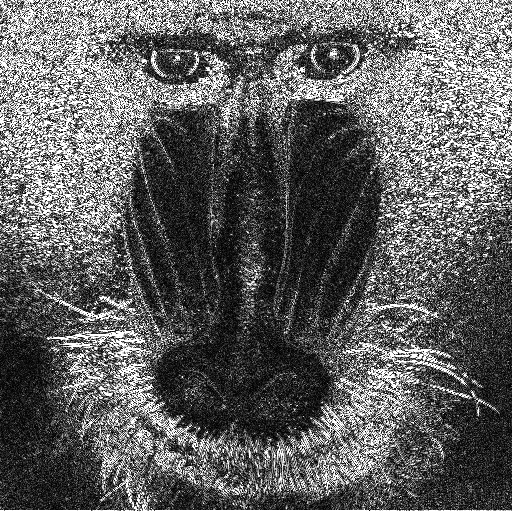
\includegraphics[width=0.9\textwidth]{imagens/baboon.png}
        \caption{Original: \texttt{baboon.png}.}
    \end{subfigure}\\[8pt]
    \begin{subfigure}{0.48\textwidth}
        \centering
        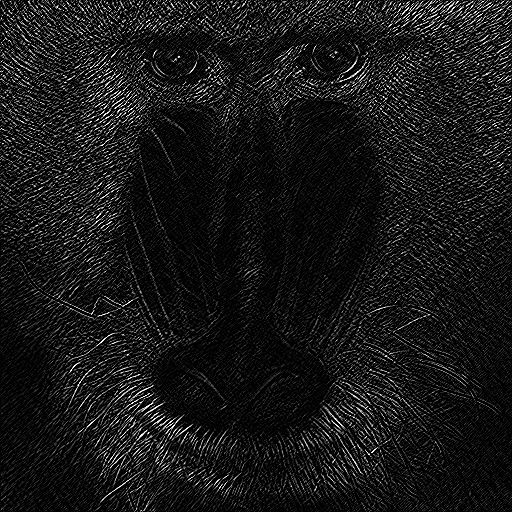
\includegraphics[width=0.9\textwidth]{resultados/baboon_h7.png}
        \caption{Convolução com ??.}
    \end{subfigure}%
    \begin{subfigure}{0.48\textwidth}
        \centering
        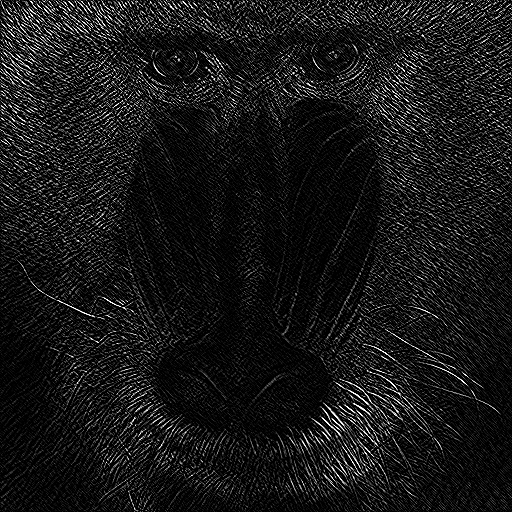
\includegraphics[width=0.9\textwidth]{resultados/baboon_h8.png}
        \caption{Convolução com ??.}
    \end{subfigure}

    \caption{??}
\end{figure}


\subsection{Sharpen} \label{sec:sharpen}

    O último filtro deste trabalho é o de nitidez, também chamado de \textit{sharpen} ou agudização. No espaço das frequências, esse tipo de filtro é responsável por enfraquecer frequências mais baixas, por isso é chamado de filtro passa-altas. Isso faz com que esse filtro seja um tipo processo "inverso" do filtro de \textit{blur} (\cref{sec:blur}).

Assim como os filtros de \textit{blur}, filtros de nitidez têm a soma de seus elementos igual a 1. Isso faz com que o aspecto geral das intensidades da imagem seja mantido. Outra característica interessante desses filtros, é que eles são basicamente uma soma do resultado de um filtro de detecção de borda não direcional com a imagem original. Podemos ver isso comparando as figuras \ref{fig:sharpen:edge}, que é a aplicação do laplaciano em \texttt{city.png}, e \ref{fig:sharpen:sub}, a subtração de \cref{fig:sharpen:sharpen} por \ref{fig:sharpen:orig}.

\begin{figure}[H]
    \centering
    \begin{kmatrix}
    \matrix(img)[square matrix]{
        -1 & -1 & -1 & -1 & -1 \\
        -1 & 2 & 2 & 2 & -1 \\
        -1 & 2 & 8 & 2 & -1 \\
        -1 & 2 & 2 & 2 & -1 \\
        -1 & -1 & -1 & -1 & -1 \\
    };

    \node[left=of img] {$\displaystyle\Scale[1.7]{\frac{1}{8}}$};
\end{kmatrix}

    \caption{Máscara de nitidez: $h_{10}$.}
    \label{fig:h10}
\end{figure}

\begin{figure}[H]
    \centering
    \begin{subfigure}{0.48\textwidth}
        \centering
        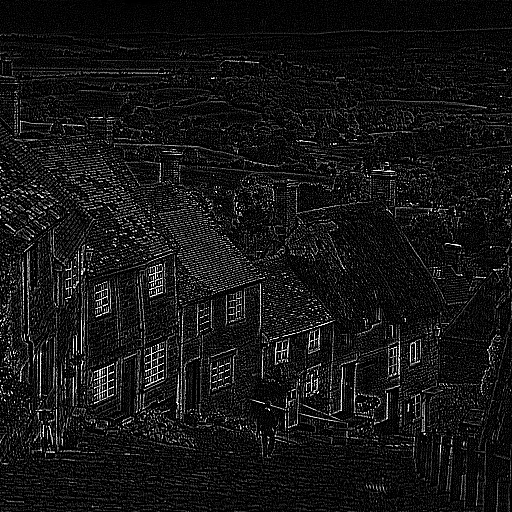
\includegraphics[width=0.9\textwidth]{imagens/city.png}
        \caption{Original: \texttt{city.png}.}
        \label{fig:sharpen:orig}
    \end{subfigure}%
    \begin{subfigure}{0.48\textwidth}
        \centering
        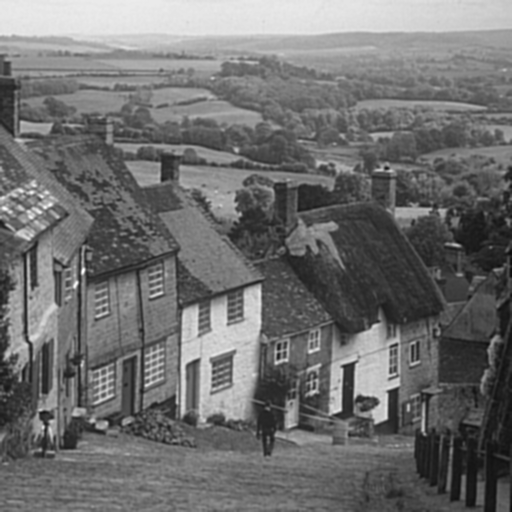
\includegraphics[width=0.9\textwidth]{resultados/city_h2h10.png}
        \caption{Convolução com $h_2$, depois com $h_{10}$.}
        \label{fig:sharpen:combinada}
    \end{subfigure}\\[8pt]
    \begin{subfigure}{0.48\textwidth}
        \centering
        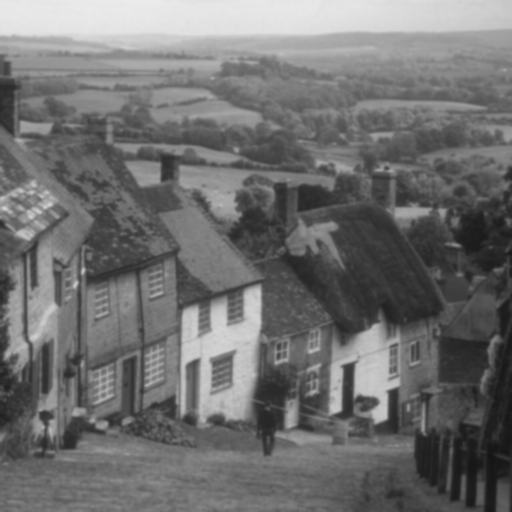
\includegraphics[width=0.9\textwidth]{resultados/city_h2.png}
        \caption{Convolução com $h_2$ (\ref{fig:h2}).}
        \label{fig:sharpen:blur}
    \end{subfigure}%
    \begin{subfigure}{0.48\textwidth}
        \centering
        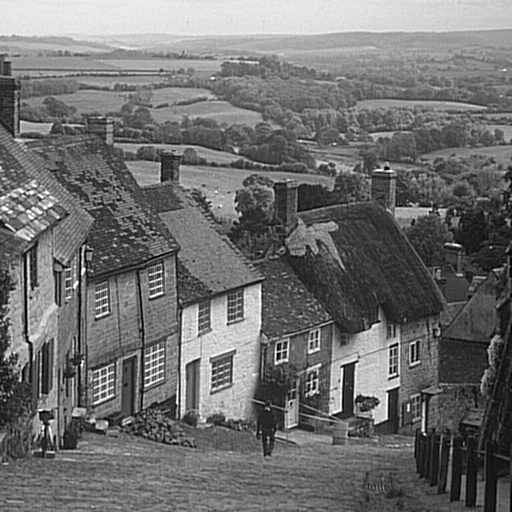
\includegraphics[width=0.9\textwidth]{resultados/city_h10.png}
        \caption{Convolução com $h_{10}$ (\ref{fig:h10}).}
        \label{fig:sharpen:sharpen}
    \end{subfigure}\\[8pt]
    \begin{subfigure}{0.48\textwidth}
        \centering
        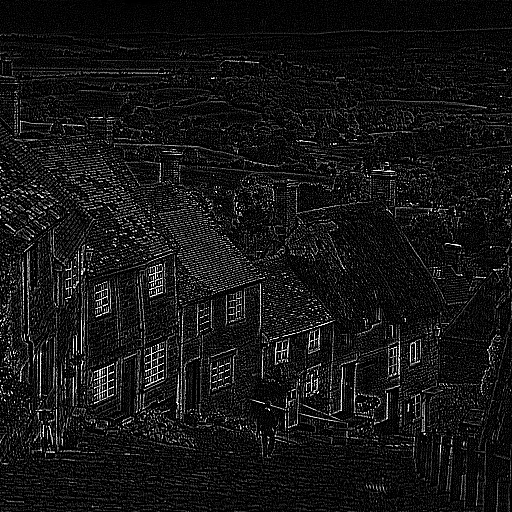
\includegraphics[width=0.9\textwidth]{resultados/city_h5.png}
        \caption{Convolução com $h_5$ (\ref{fig:h5}).}
        \label{fig:sharpen:edge}
    \end{subfigure}%
    \begin{subfigure}{0.48\textwidth}
        \centering
        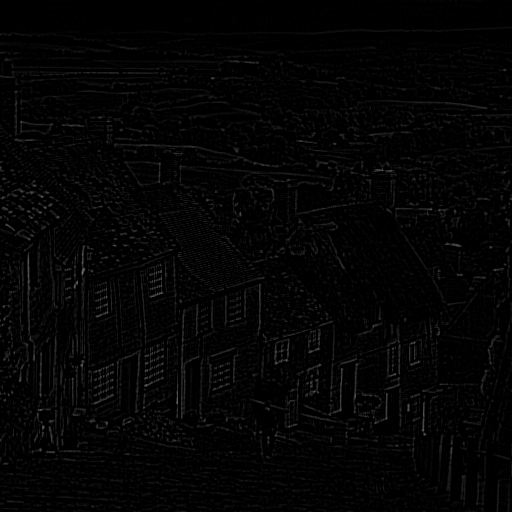
\includegraphics[width=0.9\textwidth]{resultados/city_h10e.png}
        \caption{Convolução com $h_{10}$, removido da original.}
        \label{fig:sharpen:sub}
    \end{subfigure}

    \caption{Filtros de \textit{blur} e de nitidez.}
\end{figure}

Podemos ver nas figuras \ref{fig:sharpen:blur} e \ref{fig:sharpen:sharpen}, comparando com a original (\ref{fig:sharpen:orig}), que o \textit{blur} ($h_2$) reduz a nitidez, enquanto o \textit{sharpen} ($h_{10}$) aumenta. Aplicando o filtro $h_2$ e o $h_{10}$, nessa ordem, resulta na \cref{fig:sharpen:combinada}, que tem nitidez comparável com a original.

A execução desse filtro é pode ser feita com:

\begin{minted}{bash}
    $ python3 main.py imagens/city.png h10
\end{minted}


\subsection{Gradiente} \label{sec:grad}

    Além do operador de Sobel, existem vários outros operadores baseados em gradiente. Um deles é o de Prewitt \autocite{ref:prewitt}, caracterizado por dois \textit{kernels} $3 \times 3$, com apenas $0$, $1$ e $-1$. No caso da \cref{fig:h11}, o gradiente está apontando para a direção $(-1, -1)$, isto é, da direita-inferior para a esquerda-superior.

Na \cref{fig:grad}, podemos ver claramente o direcionamento pelas antenas da borboleta. A antena esquerda, que está alinhada com o filtro, fica quase indetectada pelo filtro, enquanto a antena direita aparece de forma bem marcada. Além disso, na antena direta, apenas uma das bordas fica marcada, isso porque o filtro não depende apenas da angulação, mas do direcionamento positivo ou negativo naquele ângulo.

O operador de Prewitt, quando usado com direções ortogonais, também pode ser combinado como o de Sobel (\cref{sec:sobel}).

\begin{figure}[H]
    \centering
    \begin{subfigure}{0.48\textwidth}
        \centering
        \begin{kmatrix}
    \matrix[square matrix]{
        -1 & -1 & 0 \\
        -1 & 0 & 1 \\
        0 & 1 & 1 \\
    };
\end{kmatrix}

        \caption{Máscara $h_{11}$.}
        \label{fig:h11}
    \end{subfigure}%
    \begin{subfigure}{0.48\textwidth}
        \centering
        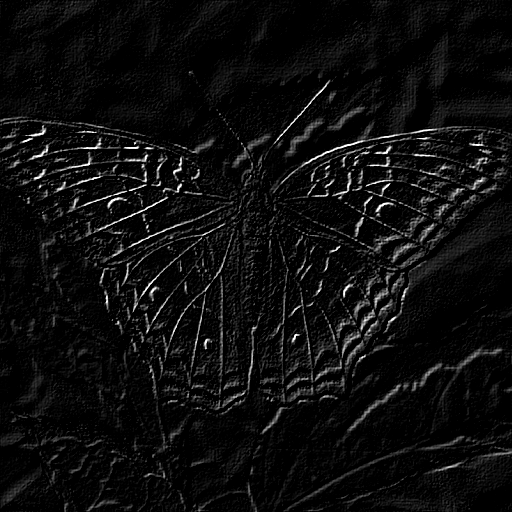
\includegraphics[width=0.9\textwidth]{resultados/butterfly_h11.png}
        \caption{Convolução com $h_{11}$.}
        \label{fig:grad}
    \end{subfigure}

    \caption{Operador de Prewitt, com exemplo.}
\end{figure}

A aplicação do filtro pode ser feita por:

\begin{minted}{bash}
    $ python3 main.py imagens/butterfly h11
\end{minted}


\subsection{Extras?}

    -n, -t, -b, --opencv


\end{document}
